\chapter{Data Structures}

This appendix summarizes, for reference purposes, all descriptor and
block layouts in Icon and Unicon.
{\color{blue}
Unicon adds extra fields to many structures in order to manage
concurrent threads and to provide mutual exclusion between
threads. These extra fields are drawn in blue.
}

\section{Descriptors}

Descriptors consist of two words (normally C ints): a d-word and a
v-word. The d-word contains flags in its most significant bits and
small integers in its least significant bits. The v-word contains a
value or a pointer. The flags are

\PrimaryIndex{Flags}%
\index{Flags!\texttt{n} flag}\index{Flags!\texttt{p} flag}%
\index{Flags!\texttt{v} flag}\index{Flags!\texttt{t} flag}%
\begin{tabular}{l@{\hspace{1cm}}l}
\texttt{n} & nonqualifier\\
\texttt{p} & v-word contains a pointer\\
\texttt{v} & variable\\
\texttt{t} & trapped variable\\
\end{tabular}

\subsection{Values}

There are three significantly different descriptor layouts for
values. A qualifier for a string is distinguished from other
descriptors by the lack of an \texttt{n} flag in its d-word, which contains
only the length of the string. For example, a qualifier for the string
{\textquotedbl}hello{\textquotedbl} is

\begin{picture}(300,40)
\put(100,0){\dvboxptr{5}{}{40}{\texttt{"hello"}}}
\end{picture}

The null value and (small) integers have type codes in their d-words and are
self-contained. Examples are:


\begin{picture}(300,40)
\put(100,0){\dvbox{null}{n}{0}}
\end{picture}

\begin{picture}(300,40)
\put(100,0){\dvbox{integer}{n}{1}}
\end{picture}


For all other data types, a descriptor contains a type code in its
d-word and a pointer to a block of data in its v-word. A record is
typical:

\begin{picture}(300,40)
\put(100,0){\dvboxptr{record}{np}{40}{block for the record}}
\end{picture}

\subsection{Variables}

There are two formats for variable descriptors. The v-word of an
ordinary variable points to the descriptor for the corresponding
value:

\begin{picture}(300,40)
\put(100,0){\dvboxptr{\textit{offset}}{npv}{40}{value descriptor}}
\end{picture}

If the variable points to a descriptor in a block, the offset is the
number of \textit{words} from the top of the block to the value
descriptor. If the variable points to a descriptor that corresponds to
an identifier, the offset is zero.


The descriptor for a trapped variable contains a type code for the
kind of trapped variable in its d-word and a pointer to the block for
the trapped variable in its v-word. The trapped variable may either be
a substring or a table element. Both are drawn in section A.2.9.

\section{Blocks}

With the exception of the null value, integers, and strings, the data
for Icon values is kept in blocks. The first word of every block is a
title that contains the type code for the corresponding data type. For
blocks that vary in size for a particular type, the next word is the
size of the block in bytes. The remaining words depend on the block
type, except that all non-descriptor data precedes all descriptor
data. With the exception of the long integer block, the diagrams that
follow correspond to blocks for computers with 32-bit words.

\subsection{Long Integers}

%% On computers with 16-bit words, integers that are too large to fit in
%% the d-word of a descriptor are stored in blocks.  For example, the
%% block for the integer 80,000 is
An Icon integer that fits in the v-word is stored there. An integer
that is too large to fit into a word is stored in a block
that is pointed to by the v-word.
The two representations of integers are distinguished by
different internal type codes: \texttt{integer} for integers that are contained
in the v-words of their descriptors and \texttt{lrgint} for integers that are
contained in blocks pointed to by the v-words of their descriptors.
Thus, there are two internal types for one source-language data type.

\begin{picture}(300,80)
\put(0,32){\dvboxptr{lrgint}{np}{60}{}}
\put(140,0){\blklrgbox{lrgint}{5,000,000,000}}
\put(140,17){\trboxlabel{title}}
\end{picture}

\subsection{Real Numbers}

Real numbers are represented by C doubles. For example, on computers
with 32-bit words, the real number 1.0 is represented by

\begin{picture}(300,80)
\put(0,32){\dvboxptr{real}{np}{60}{}}
\put(140,0){\blklrgbox{real}{1.0}}
\end{picture}

\subsection{Csets}

The block for a cset contains the usual type code, followed by a word
that contains the number of characters in the cset. Words totaling 256
bits follow, with a one in a bit position indicating that the
corresponding character is in the cset, and a zero indicating that it
is not. For example, \texttt{\&ascii} is

\begin{picture}(300,200)
\put(150,0){\blkbox{000000 ... 000000}{000000 ... 000000}}
\put(150,32){\blkbox{000000 ... 000000}{000000 ... 000000}}
\put(150,64){\blkbox{111111 ... 111111}{111111 ... 111111}}
\put(150,96){\blkbox{111111 ... 111111}{111111 ... 111111}}
\put(150,128){\blkbox{cset}{128}}
\put(150,128){\brboxlabel{size of cset}}
\put(20,144){\dvboxptr{cset}{np}{50}{}}
\end{picture}

\subsection{Lists}

A list consists of a list-header block that points to a doubly-linked
list of list-element blocks, in which the list elements are stored in
circular queues. See Chapter 6 for details. An example is the list

\iconline{ \ \ [1,2,3] }

\noindent which is represented as

\begin{picture}(300,480)
%\put(0,0){\graphpaper{30}{48}}
\put(130,0){\dvbox{null}{n}{0}}
\put(130,0){\trboxlabel{slot 3}}
\put(130,32){\dvbox{integer}{n}{3}}
\put(130,32){\trboxlabel{slot 2}}
\put(130,64){\dvbox{integer}{n}{2}}
\put(130,64){\trboxlabel{slot 1}}
\put(130,96){\dvbox{integer}{n}{1}}
\put(130,96){\trboxlabel{slot 0}}
\put(130,128){\nullptrbox{next list-element block}}
{\color{blue}
\put(-10,136){\parbox{100pt}{Unicon replaces the null pointer used by Icon
with a pointer to the list header block.}}
\multiput(100,136)(4,0){30}{\line(1,0){2}}
\put(370,136){\line(1,0){50}}
\put(420,136){\line(0,1){324}}
\put(420,460){\vector(-1,0){150}}
\put(270,460){\line(-1,0){154}}
\put(116,460){\vector(0,-1){20}}
}
\put(130,144){\nullptrbox{previous list-element block}}
\begin{picture}(0,0)(0,32)
\put(130,192){\blkbox{0}{3}}
\put(130,192){\rightboxlabels{first slot used}{number of slots used}}
\put(130,224){\blkbox{60}{4}}
\put(130,224){\rightboxlabels{size of block}{number of slots in block}}
\put(130,256){\wordbox{lelem}{}}
\put(130,288){\blkbox{}{}}
\put(130,288){\rightboxlabels{first list-element block (head)}
{last list-element block(tail)}}
{\color{blue}
\put(130,320){\wordpile{7}{\wordbox{}{}}}
\put(130,320){\brboxlabel{cvempty}}
\put(130,336){\brboxlabel{cvfull}}
\put(130,352){\brboxlabel{empty}}
\put(130,368){\brboxlabel{full}}
\put(130,386){\brboxlabel{max}}
\put(130,402){\brboxlabel{mutexid}}
\put(130,418){\brboxlabel{shared}}
}
\put(130,306){\lptr{40}}
\put(130,288){\lptr{40}}
\put(110,314){\line(0,-1){51}}
\put(110,263){\vector(1,0){20}}
\end{picture}%
\begin{picture}(0,0)(0,-80)
\put(130,320){\wordbox{\textit{id}}{}}
\put(130,336){\blkbox{list}{3}}
\put(130,336){\brboxlabel{number of elements in the list}}
\put(0,352){\dvboxptr{list}{np}{50}{}}
\end{picture}%
\end{picture}%

Here there is only one list-element block:


\subsection{Sets}

A set consists of a set-header block that contains segments that point
to blocks containing slots for linked lists of set-element blocks. 
A set header must be a proper prefix of a table header,
and a set element must be a proper prefix of a table element.
See Sec. 7.1 for details. An example is given by

\iconline{ \ \ set([100, 1, 2, 3]) }

\noindent which is represented as

\begin{picture}(300,300)(20,-30)
%set header
\put(0,72){\begin{picture}(0,0)
\put(0,96){\wordbox{7}{}}
\put(-4,96){\brboxlabel{mask}}
{\color{blue}
\put(0,112){\wordbox{}{}}
\put(-4,112){\brboxlabel{mutexid}}
\put(0,128){\wordbox{}{}}
\put(-4,128){\brboxlabel{shared}}
}
\put(0,144){\wordbox{\textit{id}}{}}
\put(0,160){\blkbox{set}{4}}
\put(-4,160){\brboxlabel{number of elements in the set}}
\put(0,0){\wordpile{5}{\nullptrbox{}}}
\put(0,80){\wordboxptr{50}{}}
\end{picture}%
}
%segment 0
\put(130,8){\begin{picture}(0,0)
\put(0,0){\nullptrbox{}}
\put(0,16){\wordboxptr{40}{}}
\put(0,32){\nullptrbox{}}
\put(0,48){\wordboxptr{50}{}}
\put(0,64){\nullptrbox{}}
\put(0,80){\nullptrbox{}}
\put(0,96){\wordboxptr{40}{}}
\put(0,112){\nullptrbox{}}
\put(0,128){\blkbox{slots}{40}}
\put(-4,128){\brboxlabel{size}}
\end{picture}%
}
\put(250,112){\line(1,0){20}}
\put(270,112){\line(0,1){120}}
\put(270,232){\vector(1,0){20}}
\put(260,64){\line(1,0){40}}
\put(300,64){\line(0,1){68}}
\put(300,132){\vector(1,0){20}}
% set element 2
\put(290,160){\begin{picture}(0,0)
\put(0,0){\dvbox{integer}{n}{2}}
\put(0,0){\brboxlabel{member value}}
\put(0,32){\wordbox{25}{}}
\put(0,32){\brboxlabel{hash number}}
\put(0,32){\brboxlabel{}}
\put(0,48){\nullptrbox{next set-element}}
\put(0,64){\wordbox{selem}{}}
\end{picture}%
}
% set element 1
\put(320,60){\begin{picture}(0,0)
\put(0,0){\dvbox{integer}{n}{1}}
\put(0,32){\wordbox{12}{}}
\put(0,32){\brboxlabel{}}
\put(0,48){\nullptrbox{}}
\put(0,64){\wordbox{selem}{}}
\end{picture}%
}
% set element 3
\put(250,-40){\begin{picture}(0,0)
\put(0,0){\dvbox{integer}{n}{3}}
\put(0,32){\wordbox{38}{}}
\put(0,32){\brboxlabel{}}
\put(0,48){\wordboxptr{40}{}}
\put(0,64){\wordbox{selem}{}}
\end{picture}%
}
% set element 4
\put(370,-56){\begin{picture}(0,0)
\put(0,0){\dvbox{integer}{n}{100}}
\put(0,32){\wordbox{1294}{}}
\put(0,32){\brboxlabel{}}
\put(0,48){\nullptrbox{}}
\put(0,64){\wordbox{selem}{}}
\end{picture}%
}
{\color[rgb]{0.7,0.7,0.7}%
\put(10,154){segment 0}
\put(30,127){\vdots}
\put(10,74){segment 5}
\put(140,124){slot 0}
\put(160,97){\vdots}
\put(140,12){slot 7}
}
\end{picture}

\subsection{Tables}

A table is similar to a set, except that a table-header block contains
the default assigned value as well as slots for linked lists of
table-element blocks. See Sec. 7.2 for details. An example is given by

\begin{iconcode}
\>t := table()\\
\>every t[98 to 100] := 1
\end{iconcode}

The table \texttt{t} is represented as

%% %--%\ \  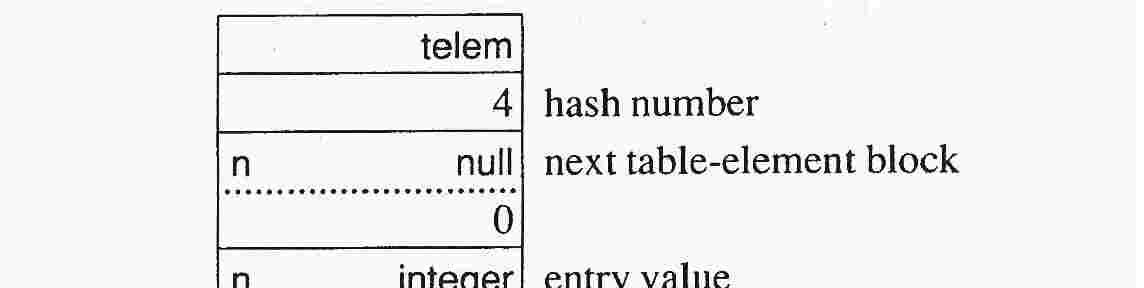
\includegraphics[width=3.848in,height=0.961in]{ib-img/ib-img122.jpg}
\begin{picture}(300,360)(20,-75)
%\put(0,-75){\graphpaper{40}{36}}
%table header
\put(0,72){\begin{picture}(0,0)
\put(0,96){\wordbox{7}{}}
\put(-4,96){\brboxlabel{mask}}
{\color{blue}
\put(0,112){\wordbox{}{}}
\put(-4,112){\brboxlabel{mutexid}}
\put(0,128){\wordbox{}{}}
\put(-4,128){\brboxlabel{shared}}
}
\put(0,144){\wordbox{\textit{id}}{}}
\put(0,160){\blkbox{table}{3}}
\put(-4,160){\brboxlabel{size of the table}}
\put(0,0){\wordpile{5}{\nullptrbox{}}}
\put(0,80){\wordboxptr{50}{}}
\put(0,-32){\dvbox{null}{n}{0}}
\end{picture}%
}
%segment 0
\put(130,8){\begin{picture}(0,0)
\put(0,0){\nullptrbox{}}
\put(0,16){\wordboxptr{40}{}}
\put(0,32){\nullptrbox{}}
\put(0,48){\wordboxptr{50}{}}
\put(0,64){\nullptrbox{}}
\put(0,80){\nullptrbox{}}
\put(0,96){\wordboxptr{40}{}}
\put(0,112){\nullptrbox{}}
\put(0,128){\blkbox{slots}{40}}
\put(-4,128){\brboxlabel{size}}
\end{picture}%
}
\put(250,112){\line(1,0){20}}
\put(270,112){\line(0,1){160}}
\put(270,272){\vector(1,0){20}}
\put(260,64){\line(1,0){40}}
\put(300,64){\line(0,1){88}}
\put(300,152){\vector(1,0){20}}
% table element 2
\put(290,200){\begin{picture}(0,0)
\put(0,-32){\dvbox{integer}{n}{1}}
\put(0,-32){\brboxlabel{assigned value}}
\put(0,0){\dvbox{integer}{n}{99}}
\put(0,0){\brboxlabel{entry value}}
\put(0,32){\wordbox{1281}{}}
\put(0,32){\brboxlabel{hash number}}
\put(0,32){\brboxlabel{}}
\put(0,48){\nullptrbox{next table-element}}
\put(0,64){\wordbox{telem}{}}
\end{picture}%
}
% table element 1
\put(320,80){\begin{picture}(0,0)
\put(0,-32){\dvbox{integer}{n}{1}}
\put(0,0){\dvbox{integer}{n}{98}}
\put(0,32){\wordbox{1268}{}}
\put(0,32){\brboxlabel{}}
\put(0,48){\nullptrbox{}}
\put(0,64){\wordbox{telem}{}}
\end{picture}%
}
% table element 3
\put(250,-40){\begin{picture}(0,0)
\put(0,-32){\dvbox{integer}{n}{1}}
\put(0,0){\dvbox{integer}{n}{100}}
\put(0,32){\wordbox{1294}{}}
\put(0,32){\brboxlabel{}}
\put(0,48){\nullptrbox{}}
\put(0,64){\wordbox{telem}{}}
\end{picture}%
}
{\color[rgb]{0.7,0.7,0.7}%
\put(10,154){segment 0}
\put(30,127){\vdots}
\put(10,74){segment 5}
\put(10,42){default value}
\put(140,124){slot 0}
\put(160,97){\vdots}
\put(140,12){slot 7}
}
\end{picture}

\subsection{Procedures}

The procedure blocks for procedures and functions are similar. For a
procedure declaration such as

\begin{iconcode}
procedure calc(i,gj)\\
\>local k\\
\>static base, index\\
\>\>\vdots\\
end
\end{iconcode}

\noindent the procedure block is


\begin{picture}(300,340)
\begin{picture}(0,0)(-100,-192)
\put(0,0){\blkboxptr{0}{40}{file name}}
\put(0,0){\trboxlabel{index of first static identifier}}
\put(0,32){\blkbox{1}{2}}
\put(0,32){\rightboxlabels{number of local identifiers}{number of static identifiers}}
\put(0,64){\wordbox{2}{}}
\put(0,64){\brboxlabel{number of arguments}}
\put(0,80){\blkboxptr{80}{40}{initial ipc}}
\put(0,80){\trboxlabel{size of block}}
\put(0,112){\wordbox{proc}{}}
\end{picture}
\put(100,0){\dvboxptr{5}{}{40}{"index"}}
\put(100,32){\dvboxptr{4}{}{40}{"base"}}
\put(100,64){\dvboxptr{1}{}{40}{"k"}}
\put(100,96){\dvboxptr{1}{}{40}{"j"}}
\put(100,128){\dvboxptr{1}{}{40}{"i"}}
\put(100,160){\dvboxptr{4}{}{40}{"calc"}}
\end{picture}


In a procedure block for a function, there is a value of -1 in place
of the number of dynamic locals. For example, the procedure block for
\texttt{repl} is


\begin{picture}(300,170)
\begin{picture}(0,0)(-100,-32)
\put(0,0){\blkbox{0}{0}}
\put(0,0){\rightboxlabels{not used}{not used}}
\put(0,32){\blkbox{-1}{0}}
\put(0,32){\rightboxlabels{function indicator}{not used}}
\put(0,64){\wordbox{2}{}}
\put(0,64){\brboxlabel{number of arguments}}
\put(0,80){\blkboxptr{40}{40}{C entry point}}
\put(0,80){\trboxlabel{size of block}}
\put(0,112){\wordbox{proc}{}}
\end{picture}
\put(100,0){\dvboxptr{4}{}{40}{"repl"}}
\end{picture}


In the case of a function, such as \texttt{write}, which has a variable number
of arguments, the number of arguments is given as -1:


\begin{picture}(300,170)
\begin{picture}(0,0)(-100,-32)
\put(0,0){\blkbox{0}{0}}
\put(0,0){\rightboxlabels{not used}{not used}}
\put(0,32){\blkbox{-1}{0}}
\put(0,32){\rightboxlabels{function indicator}{not used}}
\put(0,64){\wordbox{-1}{}}
\put(0,64){\brboxlabel{indicator of a variable number of arguments}}
\put(0,80){\blkboxptr{40}{40}{C entry point}}
\put(0,80){\trboxlabel{size of block}}
\put(0,112){\wordbox{proc}{}}
\end{picture}
\put(100,0){\dvboxptr{5}{}{40}{"write"}}
\end{picture}

\subsection{Files}

The block for a file contains a pointer to the corresponding file, a
word containing the file status, and a qualifier for the name of the
file. For example, the block for \texttt{\&output} is


\begin{picture}(300,100)
\put(120,0){\dvboxptr{7}{}{40}{\texttt{"\&output"}}}
\put(120,0){\trboxlabel{file name}}
\put(120,32){\wordbox{2}{}}
\put(120,32){\brboxlabel{file status}}
\put(120,48){\blkboxptr{file}{40}{file}}
\put(0,64){\dvboxptr{file}{np}{40}{}}
\end{picture}


The file status values are

\begin{tabular}{l@{\hspace{1cm}}l}
0 & closed\\
1 & open for reading\\
2 & open for writing\\
4 & open to create\\
8 & open to append\\
16 & open as a pipe\\
\end{tabular}

\subsection{Trapped Variables}

There are two kinds of trapped variables:
substring trapped variables, and table-element trapped variables. The
corresponding blocks are tailored to the kind of trapped variable.

A substring trapped variable contains the offset and length of the
substring, as well as a variable that points to the qpalifier for the
string. For example, if the value of \texttt{s} is
{\textquotedbl}abcdef{\textquotedbl}, the substring trapped-variable
block for \texttt{s[2:5]} is


\begin{picture}(300,170)
\put(140,0){\dvbox{}{npv}{}}
\put(140,0){\tlboxlabel{\texttt{s}}}
\put(140,0){\ruptr{30}{48}}
\put(140,48){\dvboxptr{}{npv}{50}{}}
\put(140,80){\blkbox{3}{2}}
\put(140,80){\rightboxlabels{length}{offset}}
\put(140,112){\wordbox{tvsubs}{}}
\put(10,112){\dvboxptr{tvsubs}{nptv}{50}{}}
\put(10,112){\tlboxlabel{\texttt{s[2:5]}}}
\put(270,32){\dvboxptr{6}{}{40}{\texttt{"abcdef"}}}
\end{picture}


A table-element trapped-variable block contains a word for the hash
number of the entry value, a pointer to the table, the entry value,
and a descriptor reserved for the assigned value. For example, if \texttt{t} is
a table, the table-element trapped-variable block for \texttt{t[36]} is


\begin{picture}(300,150)
\put(120,0){\dvbox{null}{n}{0}}
\put(120,0){\trboxlabel{reserved for assigned value}}
\put(120,32){\dvbox{integer}{n}{36}}
\put(120,32){\trboxlabel{entry value}}
\put(120,64){\dvboxptr{table}{np}{40}{table header block for t}}
\put(120,96){\blkbox{tvtbl}{36}}
\put(120,96){\brboxlabel{hash number}}
\put(0,112){\dvboxptr{tvtbl}{nptv}{40}{}}
\end{picture}

\subsection{Co-Expressions}

A co-expression block consists of heading information, an array of
words for saving the C state, an interpreter stack, and a C stack:

\begin{picture}(300,440)
\put(104,10){\makebox[100pt]{C stack}}
\put(100,32){\updownbars}
\put(104,52){\makebox[100pt]{interpreter stack}}
\put(100,80){\updownbars}
\put(104,100){\makebox[100pt]{cstate}}
\put(100,136){\downbars}
\put(100,136){\blkbox{}{}}
\put(100,136){\rightboxlabels{cstate[0] (saved C {\em sp})}{cstate[1]}}
\put(100,168){\dvboxptr{refresh}{np}{40}{refresh block}}
\put(100,200){\dvbox{null}{n}{0}}
\put(100,200){\trboxlabel{most recent activator}}
\put(100,232){\blkbox{}{}}
\put(100,232){\rightboxlabels{saved sp}{pointer to transmitted value}}
\put(100,264){\blkbox{}{}}
\put(100,264){\rightboxlabels{saved line number}{saved ilevel}}
\put(100,296){\blkbox{}{}}
\put(100,296){\rightboxlabels{saved argp}{saved ipc}}
\put(100,328){\blkbox{}{}}
\put(100,328){\rightboxlabels{saved efp}{saved gfp}}
\put(100,360){\blkbox{}{}}
\put(100,360){\rightboxlabels{pointer to next co-expression block}{saved pfp}}
\put(100,392){\blkbox{coexpr}{}}
\put(100,392){\rightboxlabels{title}{size}}
\put(-20,408){\dvboxptr{coexpr}{np}{40}{}}
\end{picture}


The refresh block contains information derived from the procedure
block for the procedure in which the co-expression was
created. Consider, for example,

\begin{iconcode}
procedure labgen(s)\\
\>local i, j, e\\
\>i := 1\\
\>j := 100\\
\>e := create (s || (i to j) || ":")\\
\>\>\vdots\\
end
\end{iconcode}

For the call labgen({\textquotedbl}L{\textquotedbl}), the refresh block for \texttt{e} is

\begin{picture}(300,380)
\put(100,0){\dvbox{null}{n}{0}}
\put(100,0){\trboxlabel{value of e}}
\put(100,32){\dvbox{integer}{n}{100}}
\put(100,32){\trboxlabel{value of j}}
\put(100,64){\dvbox{null}{n}{1}}
\put(100,64){\trboxlabel{value of i}}
\put(100,96){\dvboxptr{1}{}{40}{"L"}}
\put(100,96){\trboxlabel{value of s}}
\put(100,128){\dvboxptr{proc}{n}{40}{procedure block}}
\put(100,128){\trboxlabel{value of labgen}}
\put(100,160){\blkbox{}{}}
\put(100,160){\rightboxlabels{saved line number}{saved ilevel}}
\put(100,192){\blkbox{}{}}
\put(100,192){\rightboxlabels{saved argp}{saved ipc}}
\put(100,224){\blkbox{}{}}
\put(100,224){\rightboxlabels{saved efp}{saved gfp}}
\put(100,256){\blkbox{}{}}
\put(100,256){\rightboxlabels{saved number of arguments}{saved pfp}}
\put(100,288){\blkbox{}{3}}
\put(100,288){\rightboxlabels{initial ipc}{number of local identifiers}}
\put(100,320){\blkbox{refresh}{88}}
\put(100,320){\rightboxlabels{title}{size of block}}
\end{picture}
